\documentclass[conference, harvard, brazil, english]{sbatex}
\usepackage[utf8]{inputenc}
\usepackage{amsmath}
\usepackage{hyperref}
\usepackage{graphicx}
\graphicspath{{images/}}
\usepackage{ae}


\begin{document}
	\title{Projeto Final - Sistema de Visão Computacional para Futebol de Robôs}
	\date{04-07-2016}
	\author{Samuel Venzi Lima Monteiro de Oliveira\\14/0162241}{samuel.venzi@me.com}
		\twocolumn[
			\maketitle
			\selectlanguage{brazil}
		]
	
	\pagenumbering{arabic}
	
	\section{Abstract}
		\paragraph{}
		Visando melhorar os resultados da equipe de competição de futebol de robôs \textit{UnBall}, um sistema completo de visão computacional foi desenvolvido com o objetivo de fazer a detecção automática do campo, dos respectivos robôs de cada time e da bola. Trabalhos anteriores da equipe foram utilizados como base para desenvolver a lógica do sistema e além disso, a partir da revisão bibliográfica, diversas técnicas de segmentação e identificação já desenvolvidas foram adotadas. O sistema foi desenvolvido com base no processamento de imagens em OpenCV utilizando C++. Uma base de dados para testes foi criada e parte dela utilizada para as devidas calibrações do algoritmo. Os testes foram bem sucedidos em achar todos os elementos propostos com precisão sob condições de luz esperadas. A partir desse trabalho, pode-se, no futuro, aprimorar o sistema, adaptá-lo e otimizá-lo para outras competições.
		
	\section{Introdução}
		\paragraph{}
		Este trabalho foi realizado utilizando como base as necessidades da equipe UnBall, que compete na categoria IEEE Very Small Size de futebol de robôs. A categoria é disputada no Brasil desde 2003, e nela seis robôs, três de cada time, disputam a partida. As principais regras dizem que os robôs devem ser controlados remotamente por um computador que processa a imagem de uma câmera posicionada acima do campo. O principal objetivo das competições de robótica é desenvolver a tecnologia necessária para que em 2050, seja possível disputar um jogo contra humanos. Esse trabalho tratará do desenvolvimento do sistema de visão. Este não será somente útil a curto-prazo, para a competição, será útil para trabalhos futuros já que muitas técnicas e lógicas utilizadas aqui podem ser reaproveitadas para outras finalidades.
		\paragraph{}
		A visão computacional é parte fundamental da competição pois a estratégia de jogo depende das saídas do algoritmo da visão, como a posição dos robôs e da bola. A UnBall, anteriormente, já havia desenvolvido um sistema utilizando o Kinect, porém a falta de poder computacional para se trabalhar com imagens com profundidade atrapalhou o funcionamento do algoritmo. Esse trabalho, utiliza diversas técnicas para realizar toda a detecção dos elementos de interesse.
		\paragraph{}
		O estudo de métodos a aplicação no sistema se mostrou importante, apesar de não ter sido profundo. Técnicas como a criada por John F. Canny para detecção de bordas e o cálculo de histogramas foram adotadas como base para o algoritmo elaborado. Essas técnicas foram utilizadas com o objetivo de extrair as posições dos seis robôs presentes na partida além da bola e do campo.
		\paragraph{}
		A técnica de Canny se baseia nas variações de intensidades da imagem, onde variações abruptas, que são quantificadas por meio de derivadas da imagem, são consideradas bordas. O filtro de Canny apresenta uma boa precisão, boa detecção e sua característica de resposta mínima elimina ambiguidade na marcação das bordas.
		\paragraph{}
		Um filtro Guassiano é aplicado para eliminar parte do ruído. Um exemplo de \textit{kernel} Gaussiano de tamanho 5:
		\begin{center}
			$ K = \dfrac{1}{159}\begin{bmatrix} 
			2 & 4 & 5 & 4 & 2 \\
			4 & 9 & 12 & 9 & 4 \\
			5 & 12 & 15 & 12 & 5 \\
			4 & 9 & 12 & 9 & 4 \\
			2 & 4 & 5 & 4 & 2
			\end{bmatrix}$
		\end{center}
		\paragraph{}
		Após isso, duas máscaras de convolução para achar o gradiente de intensidade são aplicadas na imagem para as direções $x$ e $y$. Então os pontos que não são considerados partes de uma borda são removidos. A partir de outros dois parâmetros de limiar, os pixels são aceitos ou não como bordas.
		\paragraph{}
		Para análises de cor, a imagem no sistema de cores HSV (\textit{Hue}, \textit{Saturation} e \textit{Value}) é indicada por sua robustez em diferentes níveis de luminosidade. No sistema HSV, diferentemente do sistema RGB, a saturação não afeta todos os canais uniformemente, tornando fácil identificar cores pela matiz (\textit{hue}).
		\begin{figure}[h]
			\centering
			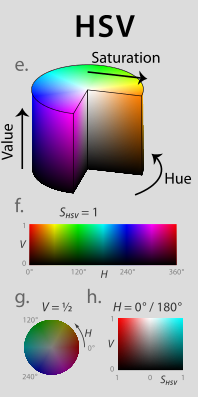
\includegraphics[scale=0.63]{hsv-2}
			\caption{Sistema HSV}
		\end{figure}
	
	\section{Metodologia}
<<<<<<< HEAD
		\paragraph{}
		Todo o desenvolvimento aconteceu com a utilização do OpenCV e com a linguagem C++. A base de dados foi criada especificamente para esse trabalho, com vídeos gravados de cima de um campo contendo seis robôs e uma bola.
		\subsection{Detecção do campo}
		\paragraph{}
		O primeiro passo do desenvolvimento foi realizar a detecção do campo, pois assim é possível criar uma região de interesse para posteriormente detectar os robôs e as bolas. Para cada frame de imagem durante o início da transmissão do vídeo foi aplicado um filtro de Canny para detecção de bordas com o objetivo de identificar as linhas que demarcam o campo. O filtro de Canny retorna uma imagem binária com as principais bordas encontradas na imagem, e um parâmetro de \textit{thresh} permite controlar os limites encontrado. A partir disso é possível encontrar os contornos e suprimir as linhas da imagem para que na região de interesse permaneçam somente os robôs. 
=======
		\subsection{Materiais}
		\paragraph{}Todo o desenvolvimento aconteceu com a utilização do OpenCV e com a linguagem C++. A base de dados foi criada especificamente para esse trabalho, com vídeos gravados acima do campo contendo seis robôs e uma bola.
		\subsection{Detecção do campo}
		\paragraph{}
		O primeiro passo do desenvolvimento é realizar a detecção do campo, pois assim é possível criar uma região de interesse para posteriormente detectar os robôs e as bolas. Cada \textit{frame} de imagem durante o início da transmissão do vídeo foi convertido em uma imagem HSV e usado apenas seu canal V, que se aproxima da imagem RBG em escala de cinza, mas com menos presença de ruídos e com valores de intensidade mais significativos. Então aplica-se um filtro de Canny para detecção de bordas com o objetivo de identificar as linhas que demarcam o campo. O filtro de Canny retorna uma imagem binária com as principais bordas encontradas na imagem, e dois parâmetros de \textit{thresh} permitem controlar os limites encontrados. À imagem binarizada é aplicada a função \textit{findcountours()} que por sua vez extrai os conjuntos de pontos que formam um contorno, em cima deste retorno é feito o tratamento de forma que apenas o maior contorno seja extraído, uma vez que este é o dado de interesse nesta etapa.
		\par Na etapa seguinte continua-se a aplicar o filtro de Canny no canal V da imagem convertida em HSV, mas com os contornos obtidos na etapa anterior subtraídos do resultado da segmentação de bordas. Tem-se assim apenas uma imagem binária com os robôs e alguns erros decorrentes do desenho não tão preciso do contorno do campo, mas por formarem linhas e não \textit{blobs} podem ser descartados no tratamento da imagem. Tais \textit{blobs} são considerados robôs e ajusta-se por meio de \textit{trackbar} qual a área minima para que um \textit{blob} seja considerado um robô. É feito também tratamento de forma a desconsiderar retângulos com a proporção maior que 1:3 ou 3:1, uma vez que os robôs tendem a formar retângulos de razão entre os lados de aproximadamente 1. Por fim, para que fique melhor definidos os blobs finais, aplica-se uma erosão na imagem binarizada final usando um kernel 2x2.
		\par A segmentação da bola é feita de maneira distinta dos robôs, por sua cor ser singular no sistema de visão e assim não aproximar-se das outras cores presentes ou possíveis é viável que se faça segmentação por cor nos \textit{frames} de entrada, para que, assim, a bola seja extraída dos outros elementos da imagem. O primeiro passo para isso é que se converta o \textit{frame} RGB da entrada para o canal HSV, de forma a amenizar a contribuição da luminosidade do ambiente na segmentação. A próxima etapa consiste em ajustar os valores dos canais H, S e V para que apenas a variação da cor laranja da bola esteja presente na imagem segmentada. Com os valores dos canais desejados, aplica-se a função \textit{inrange} resultando numa imagem com apenas um ponto branco referente ao elemento. É importante ressaltar que as duas segmentações são feitas separadamente em instâncias distintas - a segmentação dos robôs não afeta a segmentação da bola-.
>>>>>>> master
	\section{Resultados}
			
	\section{Discussão e Conclusões}
	\paragraph{}
	O sistema desenvolvido está robusto e eficiente. Os resultados mostram um sistema completamente funcional que será incluído ao algoritmo geral da equipe para trabalho junto com a estratégia de jogo. Futuramente, será adicionado ao sistema a capacidade de identificar os times automaticamente a partir das camisas dos robôs.

\end{document}